\documentclass[lang=cn,11pt,a4paper,cite=authornum]{paper}

\title{操作系统 实验:进程同步控制 \\ 实验报告}
\author{毛子恒 \\ 2019211397}
\institute{北京邮电大学\ 计算机学院}

\date{\zhtoday}

% 本文档命令
\nocite{*}

\begin{document}

\maketitle

\section{概览}

\subsection{实验内容}

利用信号量机制,提供读者-写者问题的实现方案,并分别实现读者优先与写者优先。

读者-写者问题的读写操作限制:

\begin{itemize}
    \item 写-写互斥:不能有两个写者同时进行写操作。
    \item 读-写互斥:不能同时有一个线程在读,一个进程在写。 
    \item 读-读允许:允许多个读者同时执行读操作。
\end{itemize}

\begin{itemize}
    \item 读者优先:在实现上述限制的同时,要求读者的操作优先级高于写者。要求没有读者保持等待除非已有一个写者已经被允许使用共享数据。
    \item 写者优先:在实现上述限制的同时,要求写者的操作优先级高于写者。要求一旦写者就绪,那么将不会有新的读者开始读操作。
    \item 读写者公平:在实现上述限制的同时,要求读者和写者的优先级相同。
\end{itemize}


\subsection{实验环境}

\begin{itemize}
    \item openEuler 20.03 64bit with ARM
    \item gcc version 7.3.0
    \item vim 8.1
\end{itemize}

\section{实验设计}

\subsection{相关API}

\begin{itemize}
    \item \mintinline{C}{int pthread_create(pthread_t *restrict thread, const pthread_attr_t *restrict attr, void *(*start_routine)(void *), void *restrict arg);}:在当前进程创建一个新线程,新线程通过唤起\mintinline{text}{start_routine}开始执行,\mintinline{text}{arg}参数被传递到\mintinline{text}{start_routine}的参数,\mintinline{text}{attr}指向的结构体的内容用来决定新线程创建时的一些参数,如果为\mintinline{text}{NULL},则采用默认参数。在该函数返回之前,新线程的ID将被存储到\mintinline{text}{thread}中。当成功时,该函数返回0。
    \item \mintinline{C}{noreturn void pthread_exit(void *retval);}:该函数终止调用它的线程,并且通过\mintinline{text}{retval}给当前进程中调用\mintinline{C}{pthread_join()}的另一个线程返回一个值。
    \item \mintinline{C}{int pthread_join(pthread_t thread, void **retval);}:该函数等待\mintinline{text}{thread}指定的线程终止,如果这个线程已经终止,则该函数立即返回。如果\mintinline{text}{retval}不是\mintinline{text}{NULL},则该函数复制目标线程给\mintinline{text}{pthread_exit()}的参数到\mintinline{text}{retval}所指向的地址。如果成功,该函数返回0。
    \item \mintinline{C}{int sem_init(sem_t *sem, int pshared, unsigned int value);}:该函数初始化一个信号量\mintinline{text}{sem}为初始值\mintinline{text}{value},\mintinline{text}{pshared}为0是,该信号量在本进程的线程之间共享。当成功时,该函数返回0。
    \item \mintinline{C}{int sem_destroy(sem_t *sem);}:该函数销毁信号量\mintinline{text}{sem}。当成功时,该函数返回0。
    \item \mintinline{C}{int sem_wait(sem_t *sem);}:该函数递减信号量\mintinline{text}{sem},如果它的值大于0,则函数立即返回;否则该进程阻塞直到信号量大于0。当成功时,该函数返回0。
    \item \mintinline{C}{int sem_post(sem_t *sem);}:该函数递增信号量\mintinline{text}{sem}。当成功时,该函数返回0。
    \item \mintinline{C}{unsigned int sleep(unsigned int seconds);}:该函数是进程睡眠\mintinline{text}{seconds}秒。完成后,该函数返回0。
\end{itemize}

\subsection{设计概述}

\begin{figure}[htbp]

    \centering
    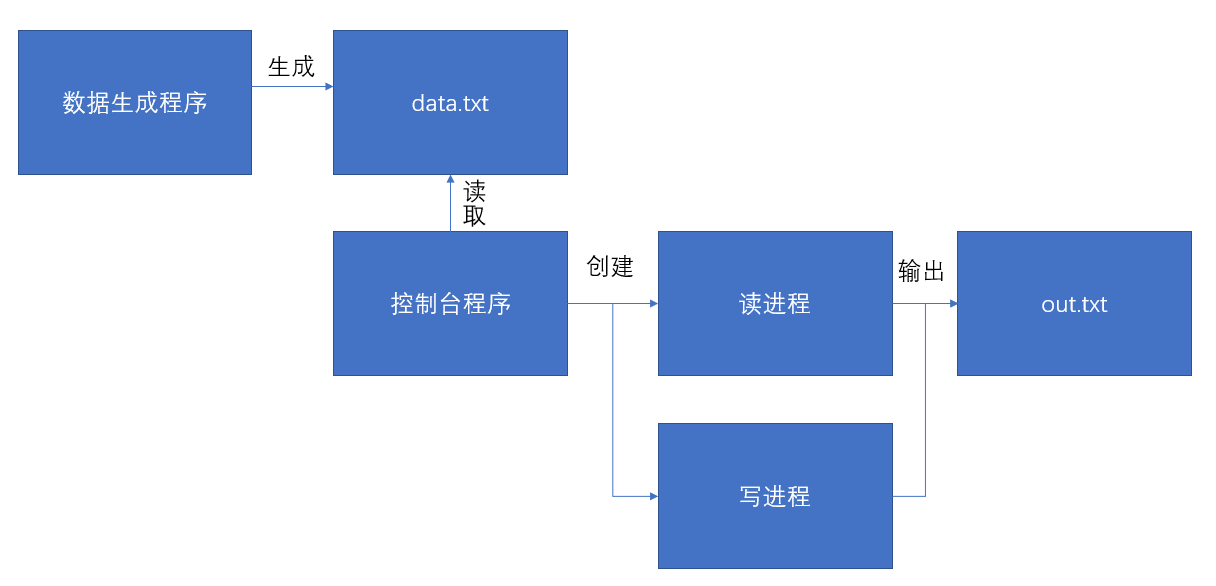
\includegraphics[width=0.8\linewidth]{./images/prog.png}
    \caption{流程图\label{fig:prog}}

\end{figure}

如\figref{fig:prog}所示,数据生成程序随机生成数据,决定读写者进程的数目、读写顺序及其读写时长,将数据写入\mintinline{text}{data.txt}中。

控制台程序从该文件中读取数据,并且分别创建读、写进程,对共享变量进行读写,将调试信息输出到标准输出中,并且将读写结果输出到\mintinline{text}{output.txt}中。

\subsubsection{读者优先}

\begin{code}
\begin{minted}{C++}
struct order
{
    char rw;
    int spendtime;
};
struct task
{
    int spendtime;
    int p_id;
    FILE *file;
};
extern int shared_data;
extern int read_count;
extern sem_t rp_wrt;
extern sem_t mutex;
void *writer(void *param);
void *reader(void *param);
void simulate(FILE *file, const std::vector<order> &orders);
\end{minted}
\end{code}

\mintinline{text}{order}结构体用于存储读写进程的信息,分别是进程类型和持续时间,\mintinline{text}{task}结构体用于给各个线程传递参数,包括持续时间、线程ID和输出的文件指针。

\mintinline{text}{shared_data}为共享变量,\mintinline{text}{read_count}为读者数量,\mintinline{text}{rp_wrt}为互斥变量,用于控制对缓冲区的访问,初始化为1,\mintinline{text}{mutex}为互斥变量,用于控制\mintinline{text}{read_count}的互斥访问,初始化为1。

写进程的逻辑如下:

\begin{code}
\begin{minted}{C++}
void *writer(void *param)
{
    sem_wait(&rp_wrt); // 等待访问权限
    /* 向 shared_data 中写入自己的线程id。*/
    sem_post(&rp_wrt); // 释放访问权限
}
\end{minted}
\end{code}

读进程的逻辑如下:

\begin{code}
\begin{minted}{C++}
void *reader(void *param)
{
    sem_wait(&mutex); // 互斥访问 read_count
    read_count++;
    if (read_count == 1) // 如果是第一个读进程,申请获取访问权限
        sem_wait(&rp_wrt);
    sem_post(&mutex);
    /* 访问缓冲区 读出 shared_data 中的信息,并输出。*/
    sem_wait(&mutex);
    read_count--;
    if (read_count == 0)
        sem_post(&rp_wrt);
    sem_post(&mutex);
}
\end{minted}
\end{code}

\subsubsection{写者优先}

\begin{code}
\begin{minted}{C++}
struct order
{
    char rw;
    int spendtime;
};
struct task
{
    int spendtime;
    int p_id;
    FILE *file;
};
extern int shared_data;
extern int read_count;
extern int write_count;
extern sem_t wp_wrt;
extern sem_t cs_read;
extern sem_t mutex_w;
extern sem_t mutex_r;
void *writer(void *param);
void *reader(void *param);
void simulate(FILE *file, const std::vector<order> &orders);
\end{minted}
\end{code}

\mintinline{text}{write_count}为写者数量,\mintinline{text}{wp_wrt}为互斥变量,用于控制对缓冲区的访问,初始化为1,\mintinline{text}{cs_read}为互斥变量,表示读者排队信号,初始化为1,\mintinline{text}{mutex_r}为互斥变量,用于控制\mintinline{text}{read_count}的互斥访问,初始化为1,\mintinline{text}{mutex_w}为互斥变量,用于控制\mintinline{text}{write_count}的互斥访问,初始化为1。

写进程的逻辑如下:

\begin{code}
\begin{minted}{C++}
void *writer(void *param)
{
    sem_wait(&mutex_w); // 互斥访问 write_count
    write_count++;
    if (write_count == 1) // 如果是第一个写进程,申请获取读进程排队权限
        sem_wait(&cs_read);
    sem_post(&mutex_w);
    sem_wait(&wp_wrt); // 申请缓冲区访问权限
    /* 向 shared_data 中写入自己的线程id。*/
    sem_post(&wp_wrt);
    sem_wait(&mutex_w);
    write_count--;
    if (write_count == 0) // 如果是最后一个写进程,释放读进程排队权限,允许其排队访问
        sem_post(&cs_read);
    sem_post(&mutex_w);
}
\end{minted}
\end{code}

读进程的逻辑如下:

\begin{code}
\begin{minted}{C++}
void *reader(void *param)
{
    sem_wait(&cs_read); // 申请排队权限
    sem_wait(&mutex_r); // 互斥访问 read_count
    read_count++;
    if (read_count == 1) // 如果是第一个读进程,申请获取访问权限
        sem_wait(&wp_wrt);
    sem_post(&mutex_r);
    sem_post(&cs_read);
    /* 访问缓冲区 读出 shared data 中的信息,并输出。*/
    sem_wait(&mutex_r);
    read_count--;
    if (read_count == 0)
        sem_post(&wp_wrt);
    sem_post(&mutex_r);
}
\end{minted}
\end{code}

\subsubsection{读写者公平}

\begin{code}
\begin{minted}{C++}
struct order
{
    char rw;
    int spendtime;
};
struct task
{
    int spendtime;
    int p_id;
    FILE *file;
};
extern int shared_data;
extern int read_count;
extern sem_t wrt;
extern sem_t cs_read;
extern sem_t mutex_r;
void *writer(void *param);
void *reader(void *param);
void simulate(FILE *file, const std::vector<order> &orders);
\end{minted}
\end{code}

\mintinline{text}{wrt}为互斥变量,用于控制对缓冲区的访问,初始化为1。

写进程的逻辑如下:

\begin{code}
\begin{minted}{C++}
void *writer(void *param)
{
    sem_wait(&cs_read);
    sem_wait(&wrt); // 申请缓冲区访问权限
    /* 向 shared_data 中写入自己的线程id。*/
    sem_post(&wrt);
    sem_post(&cs_read);
}
\end{minted}
\end{code}

读进程的逻辑如下:

\begin{code}
\begin{minted}{C++}
void *reader(void *param)
{
    sem_wait(&cs_read); // 申请排队权限
    sem_wait(&mutex_r); // 互斥访问 read_count
    read_count++;
    if (read_count == 1) // 如果是第一个读进程,申请获取访问权限
        sem_wait(&wp_wrt);
    sem_post(&mutex_r);
    sem_post(&cs_read);
    /* 访问缓冲区 读出 shared data 中的信息,并输出。*/
    sem_wait(&mutex_r);
    read_count--;
    if (read_count == 0)
        sem_post(&wp_wrt);
    sem_post(&mutex_r);
}
\end{minted}
\end{code}

\section{运行结果及分析}

\subsection{输入}

\begin{code}
\begin{minted}{text}
W 1
R 1
R 1
R 5
R 1
R 2
R 1
W 5
W 5
R 4
R 4
W 1
R 3
W 1
R 4
R 5
W 5
R 1
R 2
R 2
\end{minted}
\end{code}

\subsection{读者优先输出}

\begin{code}
\begin{minted}{text}
[ID: 1] Created thread
[ID: 1] Entering critical section
[ID: 1] Set shared_data = 1
[ID: 2] Created thread
[ID: 6] Created thread
[ID: 8] Created thread
[ID: 4] Created thread
[ID: 9] Created thread
[ID: 10] Created thread
[ID: 11] Created thread
[ID: 13] Created thread
[ID: 14] Created thread
[ID: 3] Created thread
[ID: 7] Created thread
[ID: 12] Created thread
[ID: 18] Created thread
[ID: 5] Created thread
[ID: 17] Created thread
[ID: 19] Created thread
[ID: 20] Created thread
[ID: 15] Created thread
[ID: 16] Created thread
[ID: 1] Exiting critical section
[ID: 1] Exiting
[ID: 2] Entering critical section
[ID: 2] Read shared_data = 1
[ID: 6] Entering critical section
[ID: 6] Read shared_data = 1
[ID: 10] Entering critical section
[ID: 10] Read shared_data = 1
[ID: 11] Entering critical section
[ID: 11] Read shared_data = 1
[ID: 13] Entering critical section
[ID: 13] Read shared_data = 1
[ID: 4] Entering critical section
[ID: 4] Read shared_data = 1
[ID: 7] Entering critical section
[ID: 7] Read shared_data = 1
[ID: 18] Entering critical section
[ID: 18] Read shared_data = 1
[ID: 3] Entering critical section
[ID: 3] Read shared_data = 1
[ID: 5] Entering critical section
[ID: 5] Read shared_data = 1
[ID: 19] Entering critical section
[ID: 19] Read shared_data = 1
[ID: 20] Entering critical section
[ID: 20] Read shared_data = 1
[ID: 15] Entering critical section
[ID: 15] Read shared_data = 1
[ID: 16] Entering critical section
[ID: 16] Read shared_data = 1
[ID: 2] Exiting critical section
[ID: 2] Exiting
[ID: 7] Exiting critical section
[ID: 7] Exiting
[ID: 5] Exiting critical section
[ID: 5] Exiting
[ID: 3] Exiting critical section
[ID: 3] Exiting
[ID: 18] Exiting critical section
[ID: 18] Exiting
[ID: 6] Exiting critical section
[ID: 6] Exiting
[ID: 19] Exiting critical section
[ID: 19] Exiting
[ID: 20] Exiting critical section
[ID: 20] Exiting
[ID: 13] Exiting critical section
[ID: 13] Exiting
[ID: 10] Exiting critical section
[ID: 10] Exiting
[ID: 11] Exiting critical section
[ID: 11] Exiting
[ID: 15] Exiting critical section
[ID: 15] Exiting
[ID: 4] Exiting critical section
[ID: 4] Exiting
[ID: 16] Exiting critical section
[ID: 16] Exiting
[ID: 8] Entering critical section
[ID: 8] Set shared_data = 8
[ID: 8] Exiting critical section
[ID: 8] Exiting
[ID: 9] Entering critical section
[ID: 9] Set shared_data = 9
[ID: 9] Exiting critical section
[ID: 9] Exiting
[ID: 14] Entering critical section
[ID: 14] Set shared_data = 14
[ID: 14] Exiting critical section
[ID: 14] Exiting
[ID: 12] Entering critical section
[ID: 12] Set shared_data = 12
[ID: 12] Exiting critical section
[ID: 12] Exiting
[ID: 17] Entering critical section
[ID: 17] Set shared_data = 17
[ID: 17] Exiting critical section
[ID: 17] Exiting
\end{minted}
\end{code}

\subsection{写者优先输出}

\begin{code}
\begin{minted}{text}
[ID: 1] Created thread
[ID: 1] Entering critical section
[ID: 1] Set shared_data = 1
[ID: 3] Created thread
[ID: 4] Created thread
[ID: 5] Created thread
[ID: 6] Created thread
[ID: 8] Created thread
[ID: 9] Created thread
[ID: 10] Created thread
[ID: 12] Created thread
[ID: 13] Created thread
[ID: 14] Created thread
[ID: 15] Created thread
[ID: 11] Created thread
[ID: 2] Created thread
[ID: 16] Created thread
[ID: 18] Created thread
[ID: 19] Created thread
[ID: 20] Created thread
[ID: 17] Created thread
[ID: 7] Created thread
[ID: 1] Exiting critical section
[ID: 1] Exiting
[ID: 8] Entering critical section
[ID: 8] Set shared_data = 8
[ID: 8] Exiting critical section
[ID: 8] Exiting
[ID: 9] Entering critical section
[ID: 9] Set shared_data = 9
[ID: 9] Exiting critical section
[ID: 9] Exiting
[ID: 12] Entering critical section
[ID: 12] Set shared_data = 12
[ID: 12] Exiting critical section
[ID: 12] Exiting
[ID: 14] Entering critical section
[ID: 14] Set shared_data = 14
[ID: 14] Exiting critical section
[ID: 14] Exiting
[ID: 17] Entering critical section
[ID: 17] Set shared_data = 17
[ID: 17] Exiting critical section
[ID: 17] Exiting
[ID: 3] Entering critical section
[ID: 3] Read shared_data = 17
[ID: 4] Entering critical section
[ID: 4] Read shared_data = 17
[ID: 5] Entering critical section
[ID: 5] Read shared_data = 17
[ID: 6] Entering critical section
[ID: 6] Read shared_data = 17
[ID: 10] Entering critical section
[ID: 10] Read shared_data = 17
[ID: 13] Entering critical section
[ID: 13] Read shared_data = 17
[ID: 15] Entering critical section
[ID: 15] Read shared_data = 17
[ID: 11] Entering critical section
[ID: 11] Read shared_data = 17
[ID: 2] Entering critical section
[ID: 2] Read shared_data = 17
[ID: 16] Entering critical section
[ID: 16] Read shared_data = 17
[ID: 18] Entering critical section
[ID: 18] Read shared_data = 17
[ID: 19] Entering critical section
[ID: 19] Read shared_data = 17
[ID: 20] Entering critical section
[ID: 20] Read shared_data = 17
[ID: 7] Entering critical section
[ID: 7] Read shared_data = 17
[ID: 3] Exiting critical section
[ID: 3] Exiting
[ID: 5] Exiting critical section
[ID: 5] Exiting
[ID: 7] Exiting critical section
[ID: 7] Exiting
[ID: 18] Exiting critical section
[ID: 18] Exiting
[ID: 2] Exiting critical section
[ID: 2] Exiting
[ID: 6] Exiting critical section
[ID: 6] Exiting
[ID: 19] Exiting critical section
[ID: 19] Exiting
[ID: 20] Exiting critical section
[ID: 20] Exiting
[ID: 13] Exiting critical section
[ID: 13] Exiting
[ID: 10] Exiting critical section
[ID: 15] Exiting critical section
[ID: 15] Exiting
[ID: 10] Exiting
[ID: 11] Exiting critical section
[ID: 11] Exiting
[ID: 4] Exiting critical section
[ID: 4] Exiting
[ID: 16] Exiting critical section
[ID: 16] Exiting
\end{minted}
\end{code}

\subsection{读写者公平输出}

\begin{code}
\begin{minted}{text}
[ID: 1] Created thread
[ID: 1] Entering critical section
[ID: 1] Set shared_data = 1
[ID: 3] Created thread
[ID: 4] Created thread
[ID: 2] Created thread
[ID: 7] Created thread
[ID: 8] Created thread
[ID: 10] Created thread
[ID: 11] Created thread
[ID: 12] Created thread
[ID: 13] Created thread
[ID: 14] Created thread
[ID: 5] Created thread
[ID: 6] Created thread
[ID: 9] Created thread
[ID: 15] Created thread
[ID: 20] Created thread
[ID: 16] Created thread
[ID: 17] Created thread
[ID: 18] Created thread
[ID: 19] Created thread
[ID: 1] Exiting critical section
[ID: 1] Exiting
[ID: 3] Entering critical section
[ID: 3] Read shared_data = 1
[ID: 4] Entering critical section
[ID: 4] Read shared_data = 1
[ID: 2] Entering critical section
[ID: 2] Read shared_data = 1
[ID: 7] Entering critical section
[ID: 7] Read shared_data = 1
[ID: 3] Exiting critical section
[ID: 3] Exiting
[ID: 7] Exiting critical section
[ID: 7] Exiting
[ID: 2] Exiting critical section
[ID: 2] Exiting
[ID: 4] Exiting critical section
[ID: 4] Exiting
[ID: 8] Entering critical section
[ID: 8] Set shared_data = 8
[ID: 8] Exiting critical section
[ID: 8] Exiting
[ID: 10] Entering critical section
[ID: 10] Read shared_data = 8
[ID: 11] Entering critical section
[ID: 11] Read shared_data = 8
[ID: 10] Exiting critical section
[ID: 10] Exiting
[ID: 11] Exiting critical section
[ID: 11] Exiting
[ID: 12] Entering critical section
[ID: 12] Set shared_data = 12
[ID: 12] Exiting critical section
[ID: 12] Exiting
[ID: 13] Entering critical section
[ID: 13] Read shared_data = 12
[ID: 13] Exiting critical section
[ID: 13] Exiting
[ID: 14] Entering critical section
[ID: 14] Set shared_data = 14
[ID: 14] Exiting critical section
[ID: 14] Exiting
[ID: 5] Entering critical section
[ID: 5] Read shared_data = 14
[ID: 6] Entering critical section
[ID: 6] Read shared_data = 14
[ID: 5] Exiting critical section
[ID: 5] Exiting
[ID: 6] Exiting critical section
[ID: 6] Exiting
[ID: 9] Entering critical section
[ID: 9] Set shared_data = 9
[ID: 9] Exiting critical section
[ID: 9] Exiting
[ID: 15] Entering critical section
[ID: 15] Read shared_data = 9
[ID: 20] Entering critical section
[ID: 20] Read shared_data = 9
[ID: 16] Entering critical section
[ID: 16] Read shared_data = 9
[ID: 20] Exiting critical section
[ID: 20] Exiting
[ID: 15] Exiting critical section
[ID: 15] Exiting
[ID: 16] Exiting critical section
[ID: 16] Exiting
[ID: 17] Entering critical section
[ID: 17] Set shared_data = 17
[ID: 17] Exiting critical section
[ID: 17] Exiting
[ID: 18] Entering critical section
[ID: 18] Read shared_data = 17
[ID: 19] Entering critical section
[ID: 19] Read shared_data = 17
[ID: 18] Exiting critical section
[ID: 18] Exiting
[ID: 19] Exiting critical section
[ID: 19] Exiting
\end{minted}
\end{code}

\subsection{分析}

\begin{figure}[htbp]

    \centering
    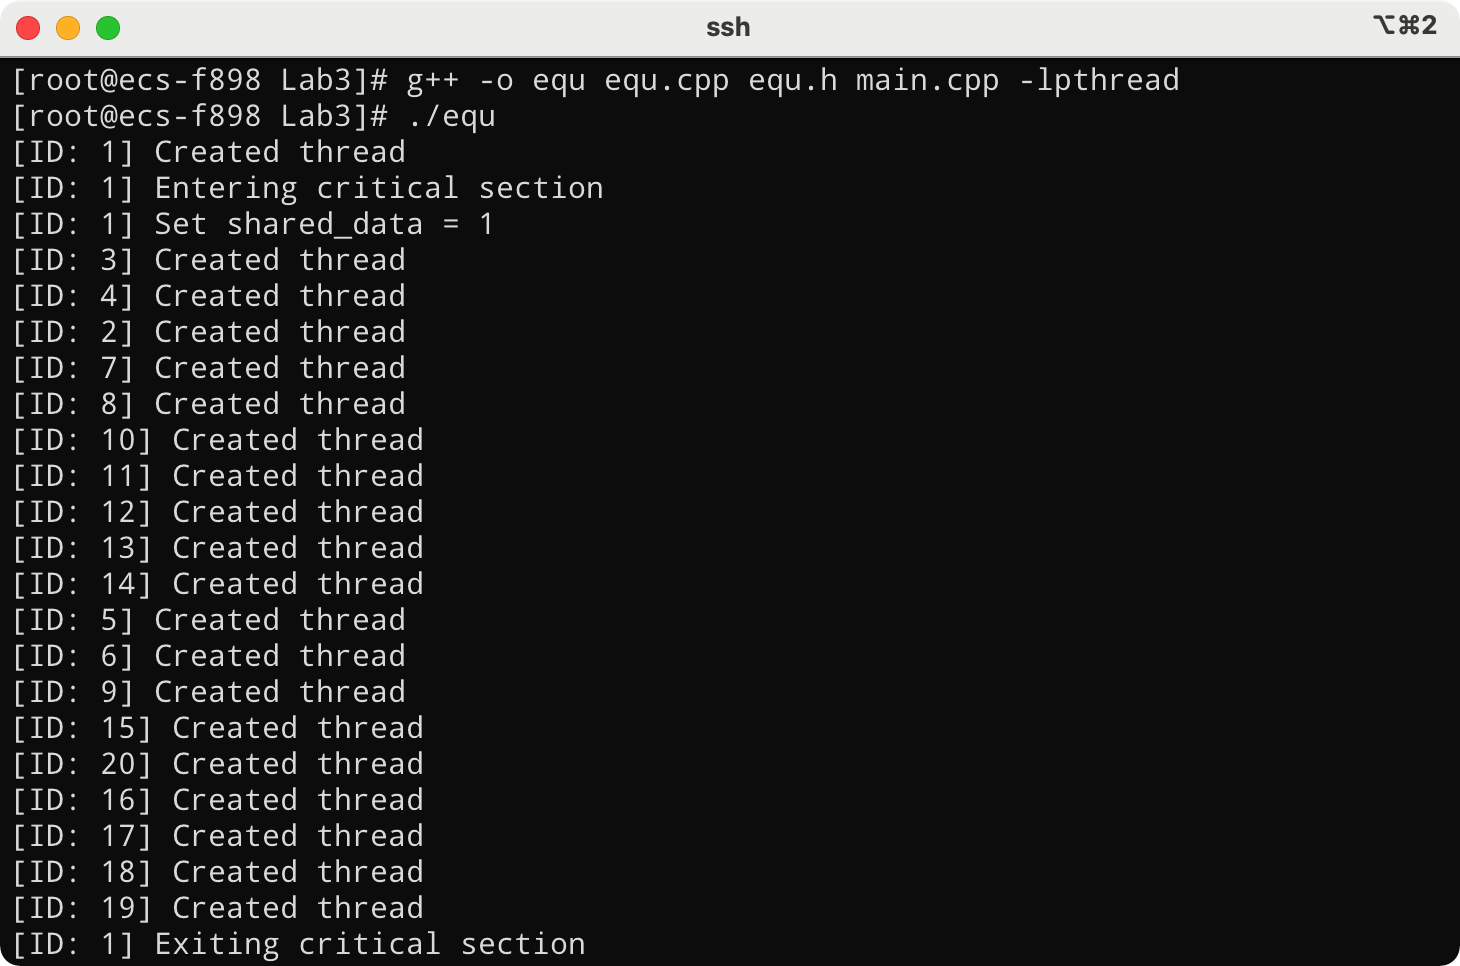
\includegraphics[width=0.6\linewidth]{./images/running.png}
    \caption{运行截图}

\end{figure}

主线程成功创建了各个工作线程,并且在各个优先级策略中,读者和写者都按照各自的优先级阻塞或运行,但是由于创建线程的顺序并不是严格依照线程ID的顺序,因此输出和预期有一些误差。总体而言程序的正确性可以保证。

\section{实验总结}

本次实验中我利用POSIX API编写了三个与进程同步控制相关的程序,使我对相关知识点的掌握更加牢固。

我通过查阅\href{https:// man7.org/linux/man-pages/index.html}{Linux man page}获取相关API的信息,并且参考教材的内容编写程序。在阅读man page和相关文档的过程中我对用户线程通过信号量进行同步的机制有了更多的认识。

本次实验使我的C编程能力和英文文献阅读能力得到提高,我从中收获颇丰。

\end{document}